% NOMENCLATURE



\chapter{Introduction}
\label{chap:1.Introduction}
\nomenclature[A]{LTA}{Lighter-than-air}
\nomenclature[A]{UAV}{Unmanned aerial vehicle}

In the last decade, unmanned aerial vehicles (UAVs) have become increasingly common in civil and commercial applications. Improvements in hardware and software have made it possible to build lightweight, energy-efficient and cost-effective vehicles with active stabilization. UAVs are particularly suited for operations beyond human reach or where human deployment poses a serious risk. Besides popular applications in media and aerial photography, tasks such as infrastructure maintenance and surveying in agriculture, wildlife monitoring and security are becoming more and more common \cite{MazurEtAl16, dro18}. Among the different UAV types, fixed-wing and multirotor vehicles are by far the most widespread and well researched. Quadcopters in particular have low entry barriers owing to their simple, transferable and inexpensive design.

Lighter-than-air (LTA) vehicles such as airships offer a distinct advantage over these platforms. Because buoyancy carries the weight of the vehicle, an airship does not have to spend energy to stay in the air. This allows considerably longer flight times than multirotors, which must produce thrust continuously, and makes airships well suited for long-duration tasks such as inspection, monitoring and surveying. Also its low speed and soft structure reduce the risk of damage to people and the environment during operation close to infrastructure. These advantages come at a price. Above all, their large volume in relation to their mass makes them highly susceptible to wind, so that controllers capable of handling strong disturbances require substantially more development effort.

Atmospheric wind is one of the dominant sources of disturbance for lighter-than-air vehicles. Airships are characterized by their large volume, low flight speed and high aerodynamic drag, which makes them considerably more susceptible to atmospheric disturbances than conventional fixed-wing aircraft or multirotors. Even moderate wind speeds can be comparable to the airspeed the vehicle is able to achieve, so that the wind may push the airship off its desired trajectory or exceed the available control authority. This sensitivity is one of the main challenges for autonomous airship operation, in particular during low-speed maneuvers such as hovering, station keeping, inspection tasks and precision landing, where the demands on tracking accuracy are highest.

Knowing the current wind is therefore valuable, but it is not directly available. A dedicated wind sensor, such as a pitot tube or an ultrasonic anemometer, can in principle measure the relative airflow, but it is often not a practical solution, especially for small autonomous airships. Additional sensors increase weight, cost and system complexity, and payload is scarce on a lighter-than-air vehicle. Pitot-based sensors also lose accuracy at the low airspeeds at which airships typically operate. Consequently, it is desirable to estimate the wind onboard from the measurements that are available anyway, such as velocity, attitude and angular rates. Such an estimator provides the wind information without additional hardware and can also be used to complement or validate a sensor if one is installed.

A reliable wind estimate enables more than observing the surrounding atmosphere. If it is fed into the flight controller, the aerodynamic disturbance can be compensated actively instead of being left for the feedback loop to reject after it has already caused a tracking error. A purely feedback-based controller reacts only to deviations that have already occurred, and for a slowly responding vehicle like an airship this delay is significant. Wind compensation has the potential to improve trajectory tracking, reduce the control effort and increase the robustness of autonomous flight under varying environmental conditions.

Achieving accurate wind estimation and effective compensation is, however, challenging. The airship dynamics are strongly nonlinear and are governed by the interaction of gravitational, buoyancy, propulsion and aerodynamic forces, while the aerodynamic effects depend on the unknown wind itself. Both the estimator and the controller must therefore take the nonlinear dynamics and the coupling between vehicle motion and surrounding airflow into account. Model-based estimators address this by exploiting a physical description of the vehicle, but their accuracy depends on the quality of the model. Data-driven methods, in contrast, learn the relation between the measurements and the wind directly from data and do not require an explicit wind model, although they depend on the available training data and on how well they generalize to conditions not seen during training.

This motivates the objectives of this work, which are outlined in the following section.


\section{Aim of this work}
\label{sec:Aim}
- Objectives
- Scope
- Evaluation scenarios

The aim of this work is to develop and implement model-based and data-driven algorithms for wind estimation and wind compensation for an unmanned airship. The proposed approach shall reliably estimate the ambient wind using only the available onboard measurements and the nonlinear dynamic model of the vehicle, without requiring dedicated wind sensors.

The wind estimation algorithm is designed to operate under conditions representative of realistic flight scenarios. These include dynamic wind conditions with gusts of up to 30 km/h, as well as different flight maneuvers such as forward and sideward flight, rotation about the vertical axis, and coordinated turning during forward flight. The estimated wind shall remain accurate and robust despite the nonlinear vehicle dynamics and changing operating conditions.

Based on the estimated wind, a model-based compensation strategy is implemented to directly counteract the aerodynamic disturbances acting on the airship. By incorporating the estimated wind into the control system, the influence of wind on the vehicle motion is reduced as directly as possible, thereby improving trajectory tracking performance and the overall robustness of the flight controller.

To evaluate the proposed approach, the complete estimation and compensation framework is implemented in a MATLAB/Simulink simulation environment using a comprehensive nonlinear airship model. The performance of the estimator and the effectiveness of the compensation strategy are assessed under various wind conditions and flight maneuvers representative of realistic operating scenarios.





\section{State of the art / Related work}
\label{sec:RelatedWork}
- Airship dynamics
- Wind estimation
- Wind compensation / disturbance observers
- Positioning this thesis





\section{Airship squid}

This work is carried out on the airship Squid, an airship developed and built by roboloon in Stuttgart. Squid features a novel propulsion system that enables omnidirectional maneuvering and is therefore well suited for the investigation of wind estimation and compensation. An overview of the airship and its main components is shown in Figure~\ref{fig:airship_squid}.

\begin{figure}[htbp]
	\centering
	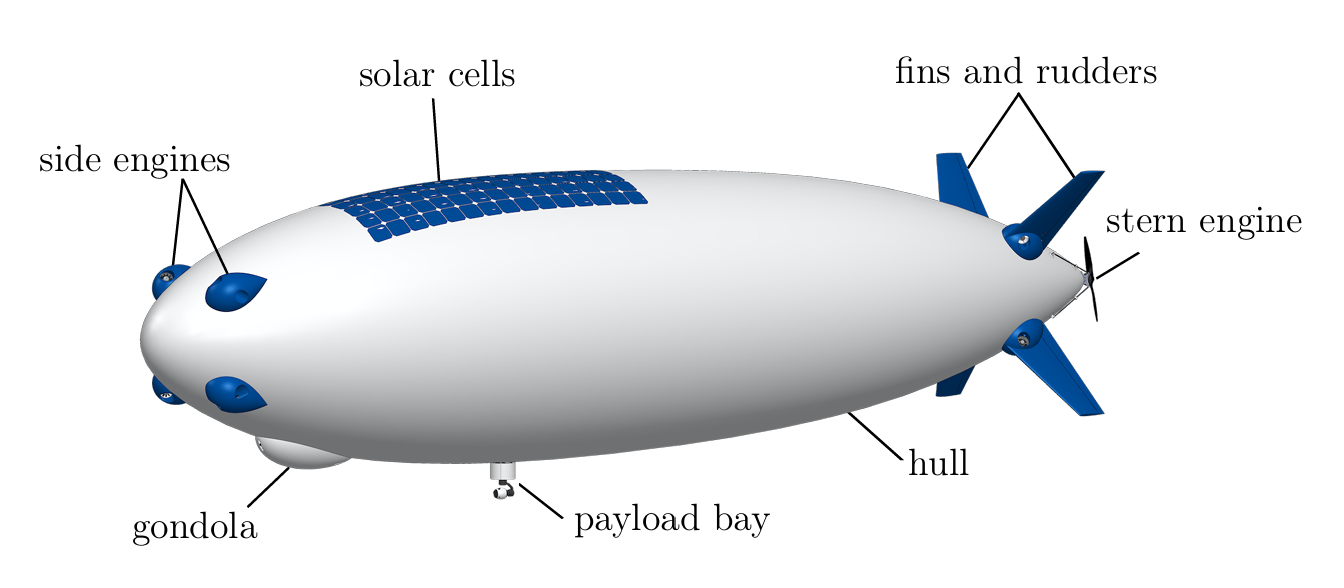
\includegraphics{src/pics/squid.png}
	\caption{CAD model of the Airship Squid and its components.}
	\label{fig:airship_squid}
\end{figure}





\subsection{Airship Configuration}
\label{sec:1.4.1Hardware}

The airship consists of an approximately \SI{8}{m} long elastic hull with a volume of \SI{16.3}{m^3}, which is filled with helium to provide the required buoyant lift. The hull is equipped with an integrated safety valve for controlled release of helium when required. The center of gravity (COG) is positioned below the center of volume (COV), while the mass is distributed approximately evenly along the longitudinal and lateral axes. This configuration provides a naturally level orientation of the airship during hovering without requiring additional control effort.

The propulsion system of the airship consists of a stern propeller, four rudders, and eight impellers with four impellers at the front and four in the back. They arranged such that their combined actuation can generate motion in all translational and rotational directions. By simultaneously actuating selected engines, the individual thrust forces can be combined to produce a desired resultant force and moment acting on the airship. This propulsion concept results in an overactuated system, as multiple combinations of actuator commands can be used to generate the same desired generalized force.

The airship is equipped with several onboard measurement systems that provide the information required for state estimation and control. The central flight-control hardware is a Cube Orange (Pixhawk~2.1), which integrates two processing units, three accelerometers, three gyroscopes, two barometers, and a compass~\cite{Cube}. In addition, an external GPS unit is connected to the flight controller and provides position and velocity measurements. The combination of the inertial, barometric, magnetic, and GPS measurements provides information on the airship's position, translational velocity, attitude, and angular rates, which form the basis for the state estimation used in the control system.

For the wind estimation investigated in this work, the airspeed measurement provides useful information on the relative wind velocity. The airship is therefore equipped with a one-dimensional Pitot tube that measures the airspeed along the body-fixed $x$-axis. The measurement is only available for airspeeds above approximately \SI{2}{m/s}. Below this threshold, no valid airspeed measurement is provided. This limitation is particularly relevant for low-speed flight and hovering conditions and is therefore taken into account in the design and evaluation of the wind estimation method.

The flight-control hardware is housed together with the battery and the remaining electrical components in the gondola located below the hull. The gondola additionally provides space for a camera and further payload. Additional sensors can be installed in the payload bay for specific applications.





\subsection{Control Architecture}
\nomenclature[A]{PID}{Proportional-integral-derivative}

The airship is controlled using a PID-based control structure. The controller receives a desired position and generates the corresponding desired forces and moments acting on the airship. The PID controller is tuned to provide robust behavior across the considered flight envelope and therefore serves as the baseline controller for this work.

The control allocator converts the desired forces and moments into individual actuator commands. Due to the overactuated propulsion system, multiple combinations of actuator inputs can produce the same desired generalized forces. The control allocator therefore determines a suitable actuator configuration while accounting for the available actuator constraints. The design and implementation of the PID controller and control allocator, including their mathematical formulation and derivation, are described in detail in \cite{Ahmed2022Controller}.

Before being implemented on the physical airship, all algorithms developed in this work are first evaluated in simulation. The simulation environment contains the airship model derived in Chapter~\ref{sec:2.2AirshipModel}, together with the implemented PID controller and control allocator. In addition to the nominal airship dynamics, uncertainties in the force and moment model are considered to account for discrepancies between the model and the physical system.

After successful validation in simulation, the algorithms are evaluated in real-world flight tests on the Airship Squid. This two-stage procedure allows the developed estimation and compensation methods to be investigated under controlled and reproducible simulation conditions before their performance is assessed on the physical airship.





